\documentclass[conference]{IEEEtran}
\usepackage{graphicx}
\usepackage{booktabs}
\usepackage{amsmath}
\usepackage{algorithm}
\usepackage{algorithmic}
\usepackage{array}
\usepackage{url}
\graphicspath{{../figures/}}
\setlength{\textfloatsep}{7pt plus 2pt minus 2pt}
\setlength{\floatsep}{7pt plus 2pt minus 2pt}
\setlength{\intextsep}{7pt plus 2pt minus 2pt}

\begin{document}

\title{Sample-Efficient PPO for CarRacing-v3 Using Road-Mask Ray Features}

\author{\IEEEauthorblockN{Joe}
\IEEEauthorblockA{Student ID: 1103820}}

\maketitle

\begin{abstract}
This project studies a sample-efficient reinforcement-learning pipeline for Gymnasium CarRacing-v3, a continuous-control driving environment where the agent receives 96 by 96 RGB observations and outputs steering, gas, and brake commands. Instead of training PPO directly on pixels, the implemented wrapper converts each frame into an HSV-based road mask, casts nine road-distance rays from a calibrated origin, and appends previous controls, speed, and a curvature proxy. Four consecutive 14-dimensional observations are stacked into a 56-dimensional vector and trained with Stable-Baselines3 PPO using MlpPolicy for 500,000 timesteps. The evaluation reloads the saved model and normalization statistics, then tests fixed COMPARE5 seeds and deterministic RANDOM10 seeds. The final artifact reaches several high-reward seeds near 900, with best raw reward 929.7, while RANDOM10 mean raw reward is 614.1 with high variance. Low-reward failure seeds remain, especially when the car drifts off road and cannot recover. The method is therefore best described as sample-efficient and promising, but not uniformly robust. RL Baselines3 Zoo is used as public configuration context only, not as a measured baseline.
\end{abstract}

\begin{IEEEkeywords}
reinforcement learning, PPO, CarRacing-v3, MLP policy, HSV road mask, ray features
\end{IEEEkeywords}

\section{Introduction}

Gymnasium CarRacing-v3 is a compact but demanding continuous-control benchmark. The observation is a 96 by 96 RGB image, while the action is a three-dimensional continuous vector for steering, gas, and brake \cite{ref1}. A pixel policy must learn visual perception, local road geometry, throttle control, and recovery behavior at the same time. That full end-to-end problem is attractive as a benchmark, but it is expensive for a course project where the training budget, hardware time, and debugging time are limited.

The environment also has a reporting challenge. A single episode can look successful for many frames and then fail suddenly after a sharp turn, off-road drift, or unstable recovery. For that reason, this report does not rely on only one best video or one best score. It evaluates the saved artifact on fixed seed sets and reports mean, variance, individual seeds, and qualitative frames. The best score shows what the policy can do, while the failure seeds show where the method still breaks.

This project takes a narrower and more reproducible path. The core idea is to keep the reinforcement-learning algorithm standard and move part of the perception burden into a deterministic image-processing wrapper. Each RGB observation is cropped, converted to HSV, thresholded into a road mask, and summarized by nine distance rays. The policy does not receive the full image. It receives a compact vector describing local road openness, recent controls, speed, and curvature. The resulting observation is small enough to train with an MLP policy rather than a convolutional image policy.

The design is intentionally conservative. It does not introduce a custom PPO variant, a new neural-network architecture, or a learned perception module. The wrapper is deterministic image processing, the learner is Stable-Baselines3 PPO, and the final evaluation reloads saved artifacts from disk. This makes the project easier to audit because the main decisions are visible: mask thresholds, ray geometry, action smoothing, reward shaping, PPO settings, normalization statistics, and evaluation seeds.

The research question is whether this compact road-geometry representation can produce useful driving behavior with a much smaller training budget than a common pixel-based PPO setup. The final model is trained for 500,000 timesteps. It is not presented as a new PPO algorithm; PPO remains the off-the-shelf learning method. The project contribution is the complete wrapper, training, evaluation, and reporting pipeline around the ray-feature representation.

The main empirical result is mixed but meaningful. Several evaluation seeds reach high reward near 900, and the best raw reward is 929.7. However, RANDOM10 mean raw reward is 614.1 with high variance, and some seeds fail with very low reward. The result supports the claim that the method is sample-efficient and promising, but it does not support a claim that the environment is solved or that the method is uniformly robust.

RL Baselines3 Zoo is used in this report as configuration context because it publishes a PPO configuration for CarRacing-v3 using image input and CnnPolicy \cite{ref5}. That context is useful for explaining why a 500,000-timestep MlpPolicy experiment is interesting. It is not a matched baseline result. The RL Zoo configuration was not re-run here under the same seed list, evaluation code, and saved-artifact protocol, so this report avoids any unsupported victory claim.

The report is organized around the teacher-facing research-paper requirements. The related-work section situates PPO, Stable-Baselines3, RL Zoo, and HSV masking. The method section defines the wrapper, formulas, pseudocode, reward shaping, and PPO settings. The experimental sections then describe the evaluation protocol and analyze the COMPARE5 and RANDOM10 evidence. The final sections discuss limitations, conservative conclusions, and the reproducibility package.

\section{Related Work}

Proximal Policy Optimization (PPO) is a widely used policy-gradient method that improves stability by limiting the size of policy updates \cite{ref2}. Its clipped surrogate objective reduces destructive updates while still allowing multiple epochs of minibatch optimization over collected rollouts. This balance between implementation simplicity and practical performance is the reason PPO is often used as a first strong baseline for continuous-control tasks.

PPO is particularly suitable for this project because the action space is continuous and the final policy must output smooth steering, gas, and brake values. The algorithm can optimize stochastic continuous policies without requiring a separate value-iteration or model-learning component. In this report, PPO is treated as a reliable baseline algorithm rather than as the research contribution. The contribution is in how the observation is represented before PPO receives it.

Stable-Baselines3 provides a maintained PPO implementation, common wrappers, vectorized environments, model saving, and evaluation utilities \cite{ref3}. It also separates policy architecture from algorithm logic. CnnPolicy is designed for image observations, while MlpPolicy is designed for vector observations \cite{ref4}. Since this project converts CarRacing images into a 56-dimensional stacked feature vector, MlpPolicy is the natural policy class.

The distinction between CnnPolicy and MlpPolicy is important for interpreting the experiment. A CnnPolicy can, in principle, learn features directly from images, but it usually needs more training time and more data. An MlpPolicy is smaller and easier to train, but it depends on the input vector already containing useful task information. This project deliberately accepts that dependency and asks whether simple road-mask rays contain enough information for practical driving behavior.

RL Baselines3 Zoo provides public training recipes and tuned hyperparameters for many Stable-Baselines3 tasks \cite{ref5}. Its CarRacing-v3 PPO entry uses image-oriented preprocessing, including frame skipping, resizing, grayscale conversion, frame stacking, reward normalization, and CnnPolicy. That setup is useful as published configuration context because it represents a standard pixel-based direction. It is not used here as a direct measured score because fair comparison would require rerunning both pipelines under the same environment version and evaluation seeds.

This distinction prevents an overclaim. The RL Zoo configuration uses 4e6 timesteps and a different observation pipeline, while this project uses 500,000 timesteps and a hand-engineered vector representation. Those differences make the configurations informative but not directly comparable as final scores. The correct comparison in this report is therefore qualitative and structural: pixel-based CNN training context versus measured ray-feature MLP training in the submitted artifacts.

The feature extraction in this project uses classical color segmentation. HSV color space is commonly used for threshold-based masking because hue and saturation can isolate color regions more directly than raw RGB channels \cite{ref6}. In this implementation, grass-like pixels are detected with a fixed HSV interval and inverted to approximate a drivable road mask. This is intentionally simple: the representation is transparent, easy to audit, and tied to CarRacing visual structure.

Classical masking is not as flexible as learned visual perception, but it has two advantages here. First, it makes the observation semantics clear: long ray distances mean open road in that direction, while short distances indicate nearby boundary or non-road pixels. Second, it reduces the chance that the report hides an unexplained visual feature inside a neural network. For an image-processing course project, that transparency is useful because the preprocessing step can be inspected independently of PPO.

The broader design resembles feature engineering for reinforcement learning. Instead of asking the policy network to learn all perception from pixels, a deterministic front end converts images into task-relevant geometry. The tradeoff is clear. The agent trains faster and is easier to inspect, but it may depend on the reliability of the mask and ray design. That tradeoff is central to the method and to the limitations discussed later.

\section{Proposed Method}

\subsection{Overview}

The implemented pipeline is shown in Fig.~\ref{fig:method}. The figure is a schematic built from notebook constants, not an experimental screenshot. The wrapper receives a 96 by 96 RGB frame from CarRacing-v3, crops the bottom dashboard area by using the top 84 rows, converts the crop to HSV, and thresholds grass-like pixels with lower bound [28, 35, 35] and upper bound [92, 255, 255]. The grass mask is inverted to approximate the road. From the origin point (48, 70) in the cropped image, nine rays are cast across angles from -70 degrees to 70 degrees.

The crop removes the lower dashboard region and keeps the road area most relevant to control. The HSV threshold is designed to identify grass-like regions, not the road directly. Inverting the grass mask is a simple way to obtain an approximate road mask because the road is the dominant non-grass drivable region in CarRacing. This is not a universal segmentation method, but it matches the visual structure of the selected environment and is easy to reproduce from the constants in Table~\ref{tab:wrapper}.

The ray origin is calibrated near the car's forward position in the cropped image. Rays pointing left and right provide lateral clearance information, while the center ray and neighboring rays provide short-term forward risk information. A large distance indicates that road pixels continue in that direction; a small distance means the ray quickly encounters non-road pixels or the image boundary. This transforms a dense image into a local geometric description that an MLP can use.

\begin{figure}[t]
\centering
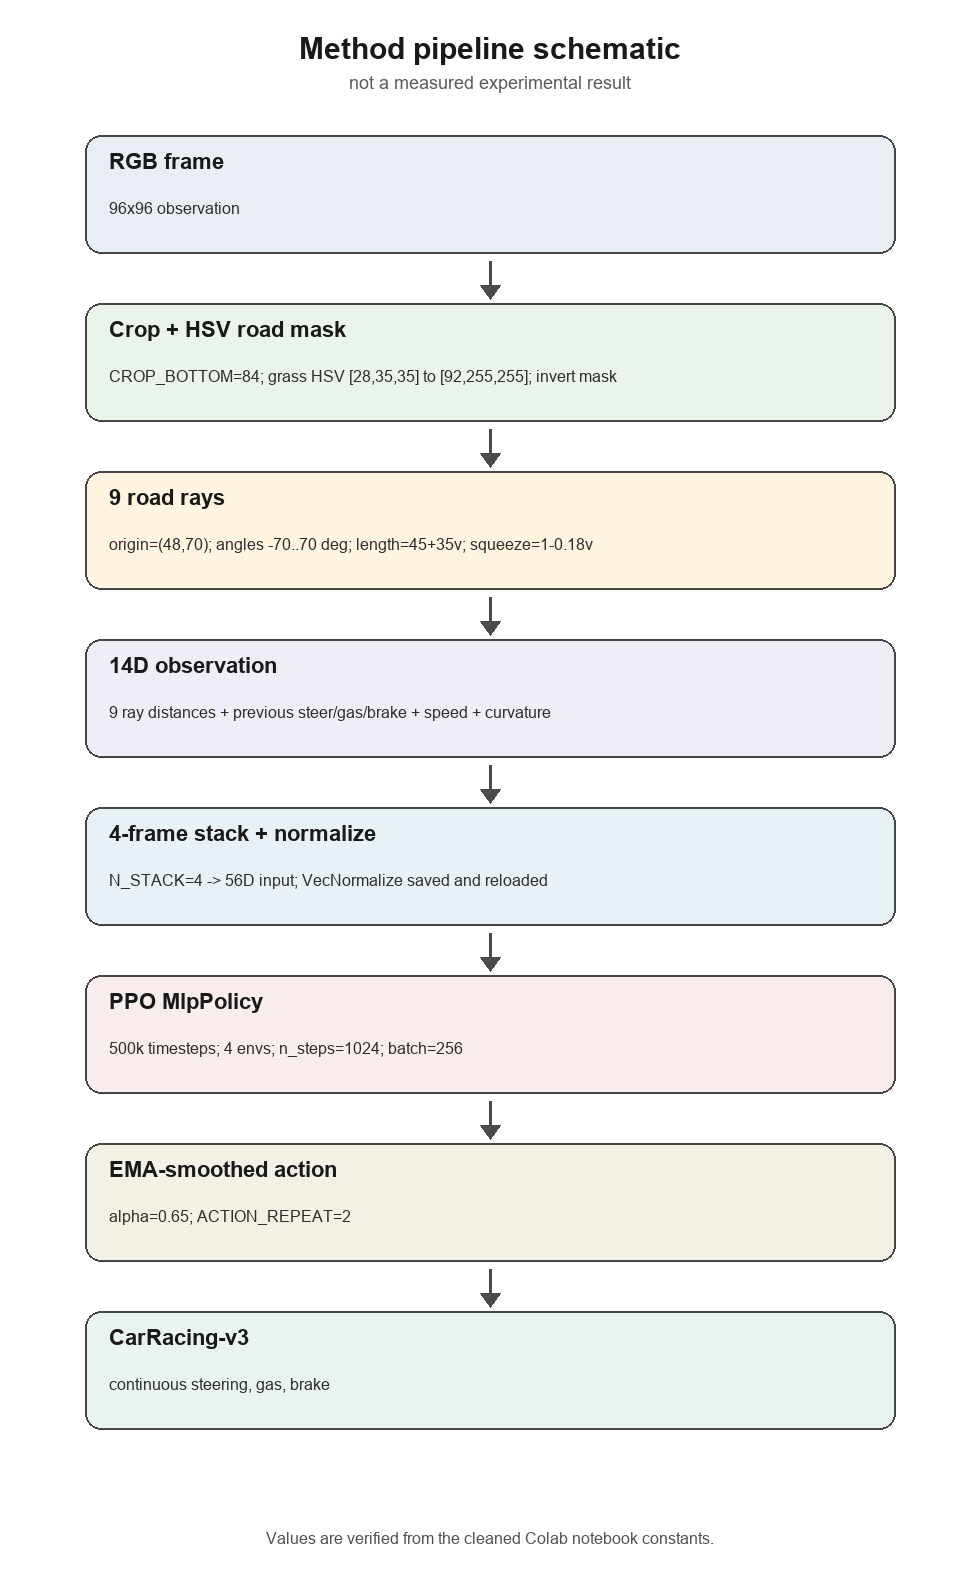
\includegraphics[width=\linewidth]{method_pipeline_schematic.png}
\caption{Implemented wrapper and training pipeline. This is a schematic based on notebook constants, not a measured experimental result.}
\label{fig:method}
\end{figure}

The ray design is speed-adaptive. The maximum ray length increases with normalized speed, and the ray angles are slightly squeezed toward the forward direction as speed increases. If the normalized speed estimate is $v_t$, the maximum ray length $\ell_t$ and adjusted angle $\alpha_i(t)$ are
\begin{equation}
\ell_t = 45.0 + 35.0 v_t,
\end{equation}
\begin{equation}
\alpha_i(t) = (1 - 0.18v_t)\beta_i,
\quad
\beta_i \in \{-70,-52.5,-35,-17.5,0,17.5,35,52.5,70\}.
\end{equation}
This makes the observation slightly more forward-looking at higher speed without changing the number of policy inputs.

\subsection{Observation Definition}

Each base observation has 14 values. The first nine are normalized ray distances. The next three are the previous smoothed steering, gas, and brake controls. The last two values are a speed estimate and a curvature proxy derived from the ray geometry. Formally, the base observation is
\begin{equation}
o_t =
[d_1,\ldots,d_9,\bar a^{steer}_{t-1},\bar a^{gas}_{t-1},
\bar a^{brake}_{t-1},v_t,c_t]\in\mathbb{R}^{14}.
\end{equation}
Four consecutive observations are stacked before being passed to the policy:
\begin{equation}
s_t = [o_{t-3},o_{t-2},o_{t-1},o_t]\in\mathbb{R}^{56}.
\end{equation}
This stack gives the MLP limited temporal context, including recent motion and control history, while keeping the input much smaller than raw pixels.

Table~\ref{tab:features} breaks down the observation layout. The table is included because the vector representation is the central method. Without this layout, the phrase ``ray features'' would be too vague to reproduce. The previous-action terms are important because CarRacing has inertia: the same road geometry can require different correction depending on whether the car was already steering, accelerating, or braking in the previous step.

\begin{table}[t]
\caption{Base Observation Layout Before Four-Frame Stacking}
\label{tab:features}
\centering
\scriptsize
\begin{tabular}{p{0.24\linewidth}p{0.20\linewidth}p{0.45\linewidth}}
\toprule
Component & Count & Meaning \\
\midrule
Ray distances & 9 & normalized local road clearance from left to right \\
Previous action & 3 & smoothed steering, gas, and brake from the previous step \\
Speed estimate & 1 & normalized movement proxy used by adaptive rays \\
Curvature proxy & 1 & road-shape signal derived from ray imbalance \\
\midrule
Total & 14 & base vector stacked over 4 frames into 56D \\
\bottomrule
\end{tabular}
\end{table}

Table~\ref{tab:wrapper} summarizes the wrapper constants verified from the cleaned notebook. These constants are reported because the method depends on the preprocessing geometry. If any of these values is changed, the trained model and saved normalization statistics should be treated as a different experiment.

\begin{table}[t]
\caption{Verified Wrapper Constants}
\label{tab:wrapper}
\centering
\scriptsize
\begin{tabular}{p{0.39\linewidth}p{0.50\linewidth}}
\toprule
Item & Value \\
\midrule
Environment & Gymnasium CarRacing-v3 \\
Crop height & CROP\_BOTTOM = 84 \\
HSV grass bounds & [28, 35, 35] to [92, 255, 255] \\
Ray origin & (48, 70) in cropped image \\
Ray angles & -70 to 70 degrees, 9 rays \\
Dynamic ray length & $45.0 + 35.0v_t$ \\
Angular squeeze & $1 - 0.18v_t$ \\
Action smoothing & EMA alpha = 0.65 \\
Action repeat & 2 environment steps \\
Stacking & 4 frames, 56D final input \\
\bottomrule
\end{tabular}
\end{table}

\subsection{Wrapper Procedure}

Algorithm~\ref{alg:wrapper} gives the wrapper logic. The important design choice is that the image processing is deterministic and external to PPO. PPO sees only the 56-dimensional state vector. During evaluation, the saved VecNormalize statistics are reloaded with the model, so the observation scale matches training.

The wrapper also keeps the final action space unchanged. The environment still receives continuous steering, gas, and brake commands. The policy's input representation changes, but the action definition remains the native CarRacing action definition. This avoids simplifying the task into a discrete-control problem and keeps the experiment aligned with the original continuous-control setting.

\begin{algorithm}[t]
\caption{Road-Mask Ray Wrapper}
\label{alg:wrapper}
\begin{algorithmic}[1]
\STATE Receive RGB frame from CarRacing-v3
\STATE Crop to the top 84 rows and convert RGB to HSV
\STATE Detect grass-like pixels using fixed HSV bounds
\STATE Invert the grass mask to obtain an approximate road mask
\STATE Estimate speed and compute adaptive ray length and angle squeeze
\STATE Cast nine rays from origin (48, 70) until non-road pixel or max length
\STATE Normalize ray distances and append previous smoothed controls, speed, and curvature
\STATE Stack four 14D observations and normalize with saved VecNormalize statistics
\STATE Feed the 56D vector to PPO MlpPolicy and smooth the continuous action
\end{algorithmic}
\end{algorithm}

\subsection{Action Smoothing and Reward Shaping}

The PPO policy outputs a continuous action vector. Before applying it to the environment, the wrapper clips it to the action bounds and applies exponential moving average smoothing:
\begin{equation}
\bar a_t = (1-\lambda)\bar a_{t-1} + \lambda \operatorname{clip}(a_t),
\quad \lambda = 0.65.
\end{equation}
The smoothed action is repeated for two environment steps. This reduces jitter and makes the controller less sensitive to single-frame feature noise. The cost is slower response during emergency recovery, which is visible in some failure cases.

Action smoothing is a practical engineering choice rather than a learning algorithm. It reduces unrealistic frame-to-frame oscillation that can appear when a compact feature vector changes sharply near road edges. However, the same smoothing can become a weakness when the car needs a sudden corrective turn or brake. The report therefore treats smoothing as part of the implemented method and recommends an ablation rather than assuming it is always beneficial.

The training reward combines the raw environment reward with shaping terms. Table~\ref{tab:reward} lists the active shaping weights from the notebook. These terms encourage road following, stable steering, and safer corner behavior. They are useful for learning within 500,000 timesteps, but they also mean the training objective is not identical to the reported raw reward. For that reason, this report uses raw reward as the headline evaluation metric and treats shaped reward as an internal training signal.

The shaping terms were chosen to support the intended behavior of the ray representation. For example, the steering guide uses road openness to encourage the car toward safer directions, while the off-road and gas-off-road penalties discourage continuing to accelerate after leaving the road. These terms do not create new environment observations; they only alter the reward used during training. The final raw-reward tables remain necessary because shaped reward can make the training curve look better than the true task reward.

\begin{table}[t]
\caption{Reward-Shaping Terms Used During Training}
\label{tab:reward}
\centering
\scriptsize
\begin{tabular}{p{0.44\linewidth}p{0.20\linewidth}p{0.25\linewidth}}
\toprule
Component & Weight & Intended effect \\
\midrule
Off-road penalty & 0.50 & discourage leaving road \\
Steering jitter penalty & 0.04 & reduce abrupt steering \\
Gas while off road & 0.10 & discourage acceleration off road \\
Steering guide & 0.15 & follow open-road direction \\
Speed bonus & 0.02 & reward forward progress \\
Curve braking bonus & 0.08 & slow for tight turns \\
Front-danger penalty & 0.20 & avoid near frontal boundary \\
Anti-spin penalty & 0.30 & reduce unstable control \\
\bottomrule
\end{tabular}
\end{table}

\subsection{PPO Objective and Settings}

The learning algorithm is standard PPO. The clipped surrogate objective is
\begin{equation}
L^{CLIP}(\theta)=
\mathbb{E}_t\left[
\min\left(r_t(\theta)\hat A_t,
\operatorname{clip}(r_t(\theta),1-\epsilon,1+\epsilon)\hat A_t\right)
\right],
\end{equation}
where $r_t(\theta)$ is the probability ratio between the new and old policies and $\hat A_t$ is the advantage estimate \cite{ref2}. This project does not modify PPO itself.

Table~\ref{tab:ppo} lists the verified PPO training settings. The policy network uses two hidden layers of 256 units for the vector observation. Four parallel environments collect rollouts. The total budget is 500,000 timesteps, which is the measured training run used for all final evaluation artifacts.

The 500,000-timestep budget is part of the experiment design. It is short compared with the 4e6-timestep RL Zoo configuration context, so the result should be interpreted as a sample-efficiency study rather than a final maximum-performance study. A longer run might improve robustness, but that would be a different experiment and is not claimed here.

\begin{table}[t]
\caption{Verified PPO Training Settings}
\label{tab:ppo}
\centering
\scriptsize
\begin{tabular}{p{0.45\linewidth}p{0.44\linewidth}}
\toprule
Item & Value \\
\midrule
Algorithm & Stable-Baselines3 PPO \\
Policy & MlpPolicy \\
Network architecture & 256 by 256 MLP \\
Total timesteps & 500,000 \\
Parallel environments & 4 \\
n\_steps & 1024 \\
Batch size & 256 \\
Gamma & 0.99 \\
GAE lambda & 0.95 \\
Entropy coefficient & 0.01 \\
Value-function coefficient & 0.5 \\
Max gradient norm & 0.5 \\
Use SDE & False \\
\bottomrule
\end{tabular}
\end{table}

\section{Experimental Setup}

All final results come from saved artifacts rather than from ad hoc notebook state. The model, VecNormalize statistics, CSV tables, figures, and evaluation videos were kept in the submission package. The cleaned notebook has its outputs and execution counts cleared, but it contains the training, artifact reload, and evaluation code needed to reproduce the workflow.

This distinction is important because reinforcement-learning notebooks can easily mix old cell state, partially trained models, and one-off evaluation code. The final workflow avoids that by separating the trained artifact from notebook execution state. The notebook can be opened cleanly, while the final results are backed by saved files: result CSVs, training evaluations, exported videos, and the saved normalization/model artifacts inside the package.

Two evaluation splits are reported. COMPARE5 uses seeds 42, 123, 777, 999, and 2026. RANDOM10 is generated from master seed 42 and contains ten deterministic seeds. Both splits reload the final model and normalization statistics before evaluation. This matters because vector observations are normalized during training; evaluating without the same normalization would change the input distribution.

Table~\ref{tab:protocol} summarizes the evaluation protocol. The table separates the reproducibility checks from the result numbers. In particular, it states that RANDOM10 is deterministic but not hand-selected seed-by-seed. This makes the split more informative than reporting only success videos, while still being small enough for a course project.

\begin{table}[t]
\caption{Final Evaluation Protocol}
\label{tab:protocol}
\centering
\scriptsize
\begin{tabular}{p{0.35\linewidth}p{0.55\linewidth}}
\toprule
Item & Protocol \\
\midrule
Artifact source & saved PPO model and saved VecNormalize statistics \\
Primary metric & raw CarRacing environment reward \\
Secondary records & shaped reward, frame count, termination label \\
COMPARE5 seeds & 42, 123, 777, 999, 2026 \\
RANDOM10 source & deterministic list from master seed 42 \\
Retraining for report & none \\
Baseline rerun & none; RL Zoo is context only \\
\bottomrule
\end{tabular}
\end{table}

Table~\ref{tab:context} describes the public RL Zoo configuration context alongside this project. The RL Zoo entry uses CnnPolicy, image preprocessing, 8 environments, and 4e6 timesteps. This project uses a 56-dimensional ray-feature stack, MlpPolicy, 4 environments, and 500,000 timesteps. The table is not a score comparison. It only explains the difference between a standard pixel-based recipe and the measured ray-feature artifact.

\begin{table}[t]
\caption{RL Zoo Configuration Context Versus This Project}
\label{tab:context}
\centering
\scriptsize
\begin{tabular}{p{0.28\linewidth}p{0.31\linewidth}p{0.31\linewidth}}
\toprule
Item & RL Zoo context & This project \\
\midrule
Role in report & public configuration & measured artifact \\
Policy & CnnPolicy & MlpPolicy \\
Input & resized grayscale image & 56D ray-feature stack \\
Frame handling & frame skip 2, stack 2 & action repeat 2, stack 4 \\
Parallel envs & 8 & 4 \\
Timesteps & 4e6 configured & 500,000 trained \\
Normalization & reward normalized & VecNormalize for features \\
Comparison status & not re-run here & evaluated here \\
\bottomrule
\end{tabular}
\end{table}

The evaluation metrics are raw reward, shaped reward, frame count, and termination label. Raw reward is the main metric because it is the native CarRacing reward. Shaped reward is included in CSV artifacts for debugging and interpretation, but it is not used to claim final performance. Termination labels such as environment done and off-road timeout help explain whether a high reward came from completing the track or from lasting through a large portion of the episode.

The reported termination labels are not treated as separate success metrics, but they help interpret reward values. An episode with a high reward and off-road timeout may still show strong driving for most of the track, while a low-reward off-road timeout indicates early failure. This is why the seed-level tables include both frames and labels rather than reward alone.

The training curve in Fig.~\ref{fig:training} was regenerated from the saved \texttt{evaluations.npz} artifact. The final multi-seed reward chart in Fig.~\ref{fig:rewards} and the seed-level tables in the next section come from the saved CSV result files. No new training or new experiment was added while preparing this report.

The experiment does not include a matched CnnPolicy baseline run. That is a limitation, but it is safer than presenting an unfair comparison. The only comparison to published resources is the RL Zoo configuration table, which describes policy type, preprocessing, training scale, and normalization settings from the public file. The measured evidence in this report belongs only to the submitted ray-feature PPO artifact.

\section{Experimental Analysis and Results}

Fig.~\ref{fig:training} shows the PPO evaluation reward during training. The curve is useful for checking that the saved model did not come from a random or untrained policy. It also shows that the learning process remains noisy, which is expected in CarRacing because track layouts and early mistakes can strongly affect total reward.

The training curve should be interpreted as diagnostic evidence rather than as the final benchmark. Evaluation during training usually uses fewer episodes than the final seed table, and it is affected by intermediate policy checkpoints. Its value is that it shows learning progress before final evaluation. The final judgment still comes from the reloaded artifact evaluated on COMPARE5 and RANDOM10.

\begin{figure}[t]
\centering
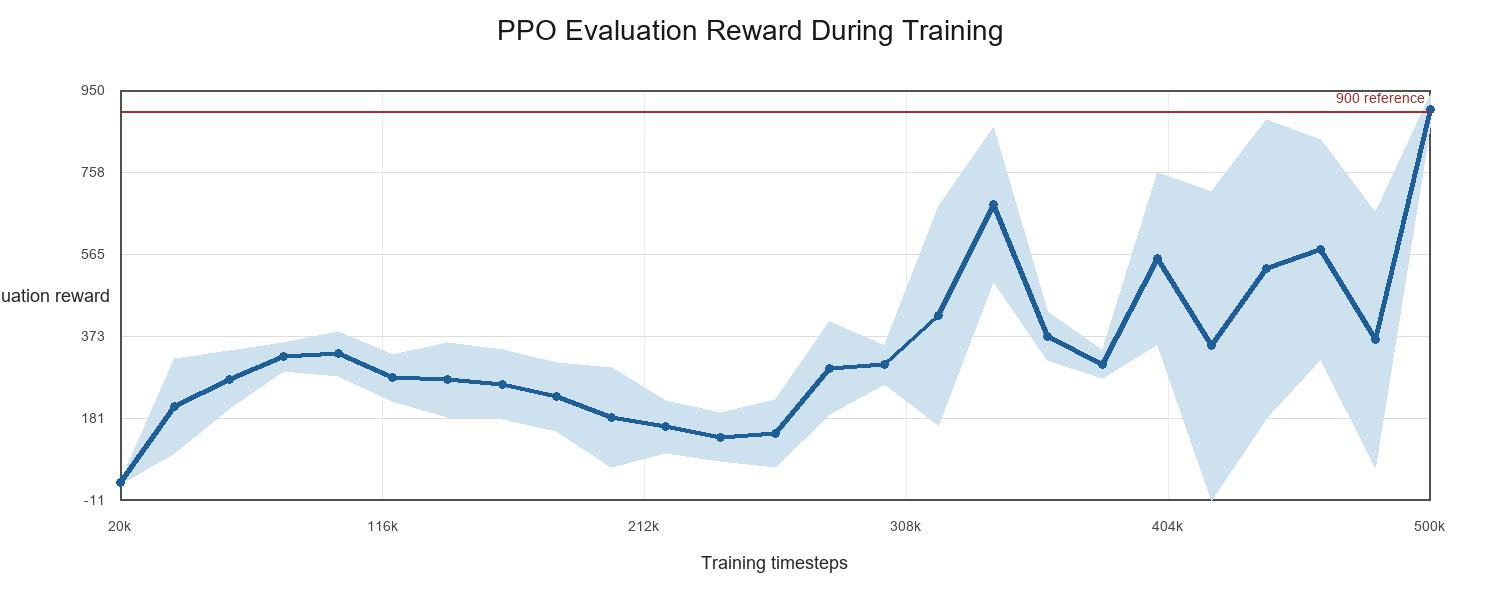
\includegraphics[width=\linewidth]{training_curve_clean.png}
\caption{PPO evaluation reward during training, regenerated from saved \texttt{evaluations.npz}.}
\label{fig:training}
\end{figure}

Table~\ref{tab:summary} summarizes the final raw reward statistics. COMPARE5 has mean raw reward 609.1 and standard deviation 348.2. RANDOM10 has mean raw reward 614.1 and standard deviation 347.8. The best raw reward is 929.7, but the minimum RANDOM10 raw reward is only 55.5. These statistics capture the central result: the method can drive very well on several seeds, but robustness is incomplete.

The two splits have similar means and standard deviations, which suggests that the RANDOM10 set does not contradict the smaller COMPARE5 set. However, both splits are high-variance. A high mean alone would hide the failure seeds, while the minimum alone would hide the strong runs. The correct reading is that the wrapper can support high-quality driving, but its reliability depends strongly on the track seed and recovery situation.

\begin{table}[t]
\caption{Final Raw Reward Summary}
\label{tab:summary}
\centering
\scriptsize
\begin{tabular}{lrrrrr}
\toprule
Split & n & Mean & Std. & Min & Max \\
\midrule
COMPARE5 & 5 & 609.1 & 348.2 & 210.8 & 896.0 \\
RANDOM10 & 10 & 614.1 & 347.8 & 55.5 & 929.7 \\
\bottomrule
\end{tabular}
\end{table}

The seed-level COMPARE5 results in Table~\ref{tab:compare5} show two low-to-medium failures and three strong runs. Seed 2026 reaches raw reward 893.33 and ends with the environment done label. Seeds 777 and 999 also reach high raw rewards, but end with off-road timeout labels. This means the policy can gather substantial track progress even when the final episode does not end perfectly.

COMPARE5 is useful because it contains seeds that were repeatedly inspected during development and final checking. It should not be treated as an unbiased estimate of generalization by itself. Its role is to provide a stable comparison set for checking whether the saved artifact behaves as expected. That is why RANDOM10 is also included.

\begin{table}[t]
\caption{COMPARE5 Seed-Level Evaluation}
\label{tab:compare5}
\centering
\scriptsize
\begin{tabular}{rrrrl}
\toprule
Seed & Raw & Shaped & Frames & Result \\
\midrule
42 & 250.42 & 219.05 & 232 & offroad timeout \\
123 & 210.82 & 191.50 & 126 & offroad timeout \\
777 & 895.95 & 853.35 & 393 & offroad timeout \\
999 & 795.11 & 761.96 & 359 & offroad timeout \\
2026 & 893.33 & 888.57 & 500 & env done \\
\bottomrule
\end{tabular}
\end{table}

Table~\ref{tab:random10} gives the RANDOM10 evidence. Four seeds reach raw rewards above 890, including the best seed 958682846 with raw reward 929.70. At the same time, seeds 599310825 and 440213415 fail very early with raw rewards 55.51 and 56.17. The final conclusion therefore cannot be based only on the best seed. The mean and the seed table must be read together.

RANDOM10 is the stronger evidence for the final claim because it includes deterministic seeds not manually selected one by one for presentation. The split contains both excellent outcomes and severe failures. In a professional report, that mixed result is more credible than reporting only the high-reward examples. It also gives a clear direction for future work: improving recovery behavior should matter more than increasing the already strong best-case score.

\begin{table}[t]
\caption{RANDOM10 Seed-Level Evaluation}
\label{tab:random10}
\centering
\scriptsize
\begin{tabular}{rrrrl}
\toprule
Seed & Raw & Shaped & Frames & Result \\
\midrule
478163327 & 902.76 & 872.19 & 402 & offroad timeout \\
107420369 & 892.03 & 871.86 & 500 & env done \\
1181241943 & 900.10 & 848.51 & 388 & offroad timeout \\
1051802512 & 458.80 & 445.09 & 206 & offroad timeout \\
958682846 & 929.70 & 934.32 & 352 & env done \\
599310825 & 55.51 & 19.98 & 85 & offroad timeout \\
440213415 & 56.17 & 34.84 & 64 & offroad timeout \\
373399426 & 554.40 & 521.07 & 273 & offroad timeout \\
1812140441 & 898.35 & 859.69 & 403 & offroad timeout \\
136505587 & 492.75 & 466.16 & 195 & offroad timeout \\
\bottomrule
\end{tabular}
\end{table}

Fig.~\ref{fig:rewards} visualizes the same final multi-seed reward distribution. The figure makes the high variance visible: strong seeds cluster around 890 to 930, while failure seeds remain near the bottom. This visual evidence supports the same interpretation as the tables and prevents the best raw reward from being overinterpreted.

The multi-seed chart also shows why the result should be described as sample-efficient. A 56-dimensional MLP policy trained for 500,000 timesteps can reach rewards close to the common 900-point success region on multiple seeds. At the same time, the chart prevents an exaggerated conclusion because the low bars are equally visible. The project is successful as a compact representation study, not as a fully robust driving solution.

\begin{figure}[t]
\centering
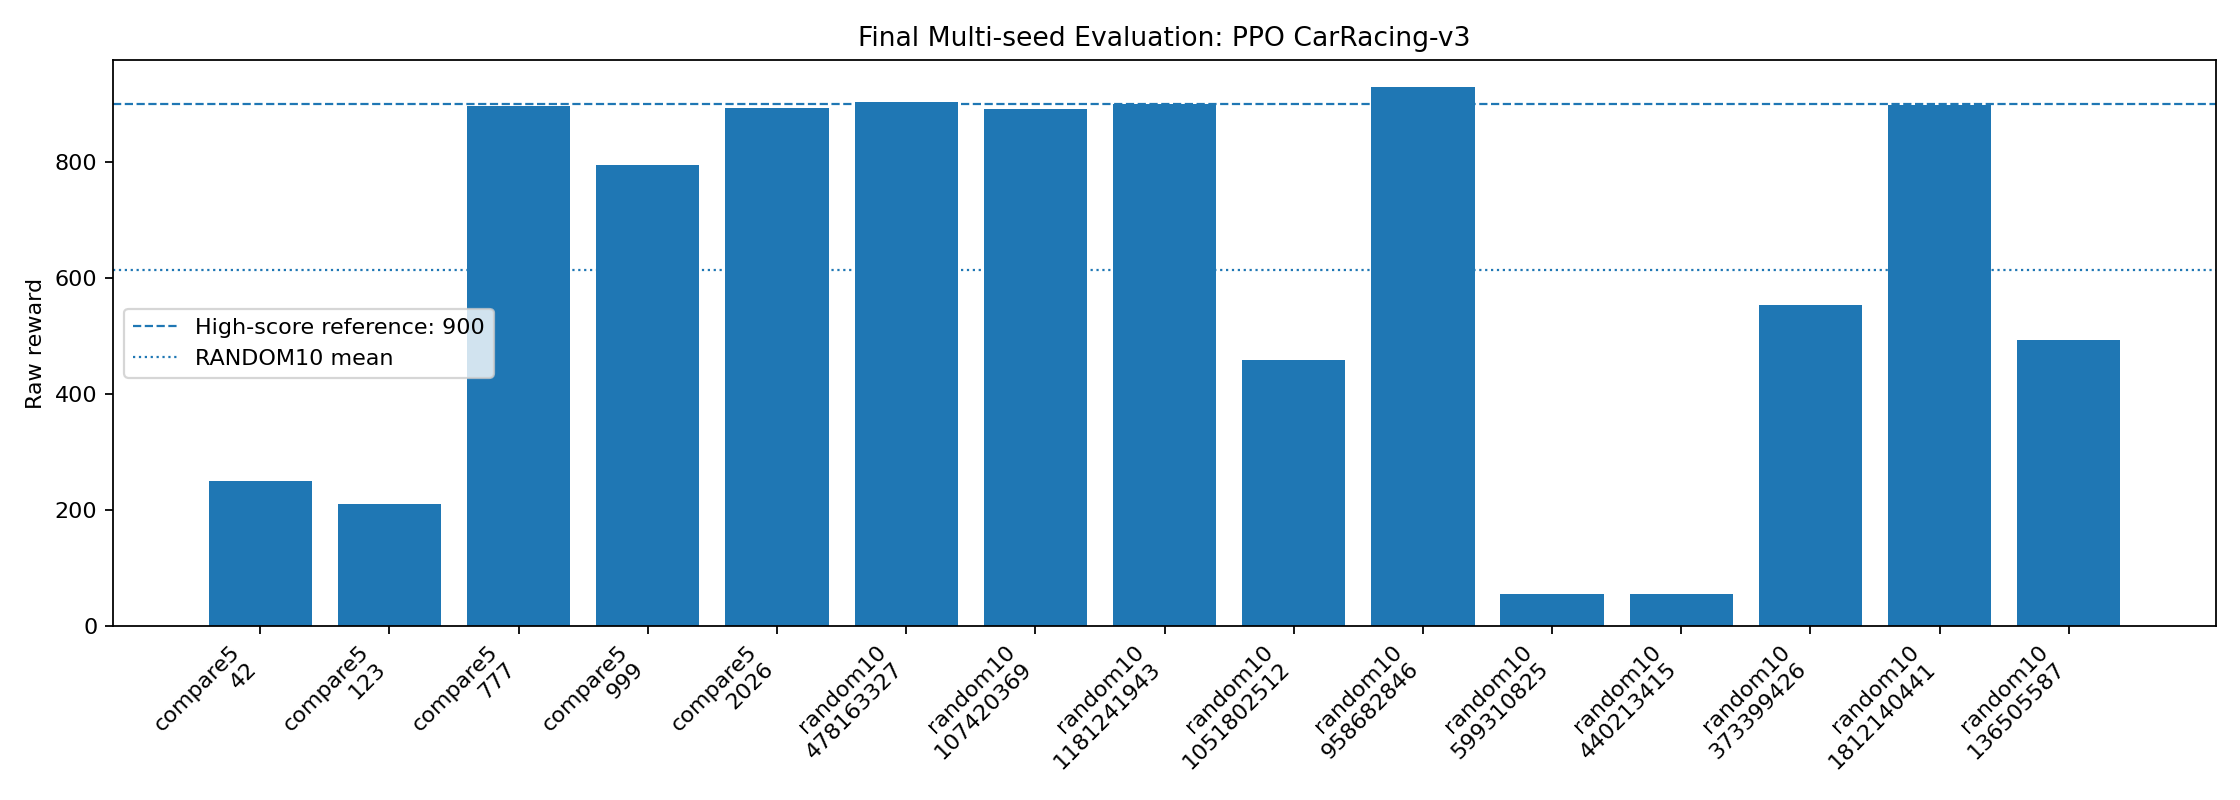
\includegraphics[width=\linewidth]{final_multiseed_rewards_clean.png}
\caption{Final raw rewards for COMPARE5 and RANDOM10 seeds. The distribution contains both high-reward runs and low-reward failures.}
\label{fig:rewards}
\end{figure}

Fig.~\ref{fig:qualitative} provides qualitative video-frame evidence. The success strip uses seed 2026 and shows the car remaining aligned through a visible road section. The failure strip uses seed 599310825 and shows an off-road drift followed by weak recovery. These frames are included to explain what the numeric failure labels look like, not to replace quantitative evaluation.

The qualitative examples are intentionally limited to one combined figure. More screenshots would make the report look fuller but would not add much evidence. The important point is that the high reward and low reward cases correspond to visibly different behavior. The success strip demonstrates useful road following, while the failure strip demonstrates the remaining weakness in recovery after leaving the road.

\begin{figure}[t]
\centering
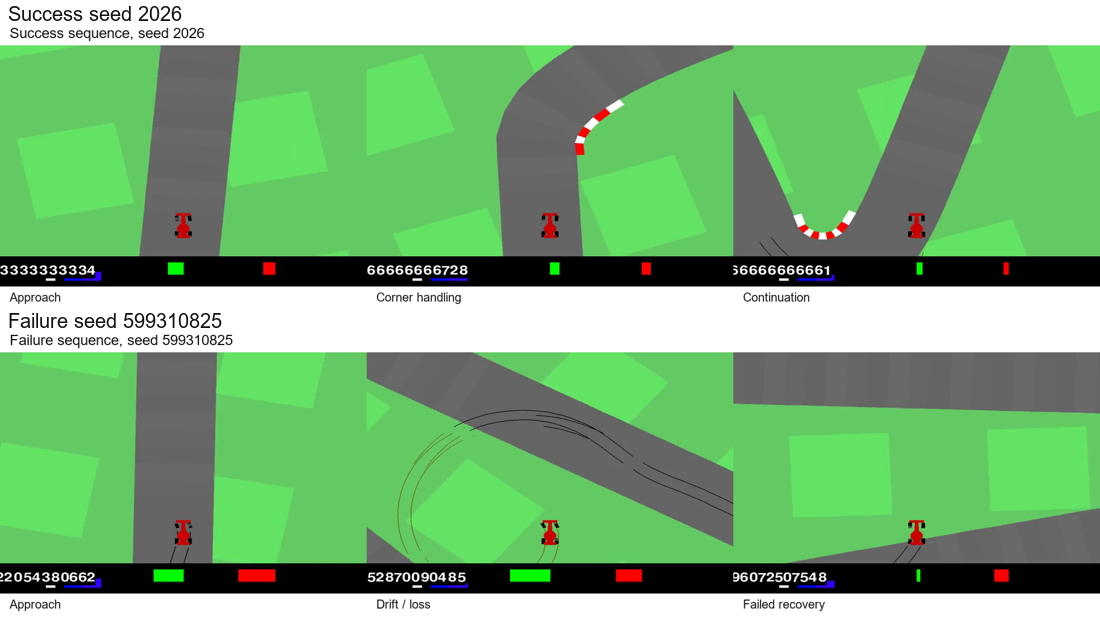
\includegraphics[width=\linewidth]{qualitative_success_failure_compact.png}
\caption{Qualitative success and failure examples from exported videos. The examples are illustrative; the quantitative evidence is in the CSV-backed tables and charts.}
\label{fig:qualitative}
\end{figure}

The strongest evidence for the method is not that every seed performs well. It is that a small vector representation trained for 500,000 timesteps can produce multiple high-reward driving episodes near 900. This suggests that road-mask ray features can capture useful local geometry for CarRacing control. The weakness is equally clear: the representation and controller still fail on certain track conditions and recovery situations.

Another important observation is that shaped reward and raw reward are close for some strong seeds but not identical. For example, seed 958682846 has raw reward 929.70 and shaped reward 934.32, while failure seed 599310825 has raw reward 55.51 and shaped reward 19.98. This difference reinforces why raw reward is the headline number. Shaped reward is useful for training analysis, but the raw score better represents the original environment objective.

The result should also be interpreted in light of action smoothing. EMA smoothing helps reduce jitter, which is useful when ray features change abruptly from frame to frame. However, smoothing can delay corrective steering or braking after the car begins to leave the road. Some low-reward failures are consistent with that tradeoff, although a controlled ablation would be needed to prove the cause.

Finally, the comparison to RL Zoo must remain conservative. RL Zoo gives a public, recognizable CarRacing PPO configuration using a larger image-based training setup \cite{ref5}. The present work shows that a much smaller engineered representation can obtain strong episodes within 500,000 timesteps, but it does not provide a direct performance comparison against the RL Zoo baseline. A fair claim would require running both methods in the same evaluation harness.

\section{Discussion and Limitations}

The main advantage of the proposed wrapper is dimensionality reduction. A raw 96 by 96 RGB frame contains 27,648 pixel values. The final stacked observation contains 56 values. This reduction makes the policy network smaller, makes the observation easier to inspect, and lets PPO spend more of its limited training budget on control instead of low-level visual feature learning.

This dimensionality reduction is the main reason the result is plausible under a 500,000-timestep budget. A pixel-based policy must learn edge, color, road-shape, and control features through gradient updates. The proposed wrapper provides a fixed road-geometry summary before learning begins. That does not make the task easy, but it changes the problem from visual representation learning plus control into mostly control from engineered geometry.

The method is also easier to explain than an end-to-end visual policy. If the agent fails, the road mask, ray distances, previous controls, and curvature feature can be inspected directly. This is useful for a course project because it connects the image-processing design to the reinforcement-learning result. The qualitative success and failure frames make this connection visible, but the actual evidence remains the saved CSV evaluation data.

The same interpretability also makes the failure modes easier to reason about. If the car is centered and the road remains visible, ray distances provide a useful steering signal. If the car points away from the road or the mask is dominated by grass after a drift, the local rays may no longer describe a good recovery path. This explains why high-reward driving and early failure can both appear in the same final model.

The first limitation is mask dependence. HSV thresholding works because the CarRacing visual environment has consistent grass and road colors. If lighting, textures, or environment rendering changed, the fixed HSV thresholds might fail. The method is therefore not a general vision solution. It is an engineered representation for this benchmark.

Mask dependence also affects reproducibility. A different CarRacing version or rendering backend could change colors enough to alter the mask. The report therefore names the environment version and the exact HSV thresholds. If a future reproduction uses different visual output, the first debugging step should be to inspect the road mask before changing PPO settings.

The second limitation is locality. Rays cast from a fixed origin describe nearby road openness, not the full future track. This can be enough for local steering, but it may be weak for long-horizon planning and recovery. Once the car leaves the road or points away from the track, the local ray pattern may not contain enough information for reliable recovery.

The third limitation is reward shaping. Shaping terms help PPO learn within the available 500,000-timestep budget, but they create a training reward different from the raw environment reward. This is why the report separates shaped reward from raw reward and uses raw reward as the main evaluation score. Future work should test how much each shaping term contributes.

Reward shaping can also hide problems during training if only shaped reward is monitored. A policy might learn to satisfy shaping terms without maximizing true track progress. The final tables reduce this risk by reporting raw reward, shaped reward, frame count, and termination label together. Still, a clean ablation without shaping would be needed to measure how much of the final performance comes from the representation alone.

The fourth limitation is the missing matched baseline. The report uses RL Zoo only as configuration context. A stronger experimental study would train the RL Zoo CnnPolicy recipe and the ray-feature MlpPolicy recipe under the same hardware, environment version, training budget variants, and seed list. That would allow direct sample-efficiency and final-performance comparisons.

This limitation is not only a matter of fairness; it is also a matter of scientific clarity. A CnnPolicy might require more timesteps but could eventually recover better because it retains full image information. The ray-feature policy may train faster but lose information needed for difficult recovery cases. A matched baseline and ablations would separate those possibilities.

Future ablations should remove or vary one component at a time: fixed ray length instead of speed-adaptive length, no angular squeeze, no previous-action inputs, no curvature proxy, no action smoothing, and no reward shaping. These ablations would identify whether the high-reward seeds are mainly due to the ray geometry, the control smoothing, the reward shaping, or their combination.

The most urgent ablation is recovery behavior. The failure seeds suggest that the method's ceiling may not be normal corner following, but returning to the road after a bad position. Future work could test longer side rays, a recovery-specific feature, or a lower action-smoothing coefficient when the front ray is short. Those changes should be evaluated carefully because they may improve failures while hurting stable high-reward seeds.

\section{Conclusion}

This project implemented a reproducible PPO pipeline for CarRacing-v3 using deterministic road-mask ray features. The RGB observation is converted into a 14-dimensional base observation, stacked into a 56-dimensional vector, normalized, and trained with Stable-Baselines3 PPO using MlpPolicy for 500,000 timesteps.

The final model demonstrates promising sample efficiency. It reaches several high-reward seeds near 900 and a best raw reward of 929.7. At the same time, RANDOM10 mean raw reward is 614.1 with high variance, and low-reward failure seeds remain. The correct conclusion is therefore balanced: the representation is effective on many seeds, but the policy is not uniformly robust.

The next step is a matched baseline and ablation study. RL Zoo currently serves as configuration context only. A direct performance claim against RL Zoo should be made only after both pipelines are trained and evaluated under the same protocol.

\section*{Data Availability and Reproducibility}

The complete source code, notebook, figures, result tables, and artifact package are available at \url{https://github.com/UltraLamb/CarRacingV3-PPO-RayFeatures}. The repository contains the cleaned Colab notebook, report source, presentation slides, result CSV files, figures, and an artifact zip with saved model-related files and evaluation data.

Table~\ref{tab:repro} lists the planned repository contents and their roles. This table is included because the course requirement asks for source code, README, installation instructions, and dataset information. The notebook is the main executable source file. The CSV files and figures are evidence files. The report source is included so the formal IEEE-style PDF can be rebuilt in Overleaf. Internal build or preview scripts are not part of the required course submission.

\begin{table}[t]
\caption{Reproducibility Package Contents}
\label{tab:repro}
\centering
\scriptsize
\begin{tabular}{p{0.34\linewidth}p{0.56\linewidth}}
\toprule
File or folder & Purpose \\
\midrule
README.md & project overview, setup, and reproduction path \\
DATASET.md & explains Gymnasium CarRacing-v3 data generation \\
requirements.txt & Python packages needed for notebook execution \\
notebooks/ & cleaned Colab notebook with training and evaluation code \\
report/ & IEEE-style LaTeX source and local PDF preview \\
slides/ & final presentation deck \\
tables/ & COMPARE5, RANDOM10, and summary CSV evidence \\
figures/ & training curve, reward chart, method schematic, qualitative frames \\
artifact zip & saved model-related files and evaluation artifacts for reload \\
\bottomrule
\end{tabular}
\end{table}

The project does not use an external downloaded dataset. Observations are generated by Gymnasium CarRacing-v3 during training and evaluation \cite{ref1}. Reproducibility depends on installing the listed Python requirements, running the cleaned notebook, preserving VecNormalize with the PPO model, and evaluating the same COMPARE5 and RANDOM10 seed lists. The artifact reload path is included so the final evaluation can be repeated without retraining.

The most important reproducibility detail is that the model and VecNormalize statistics must be used together. The policy was trained on normalized 56-dimensional observations, so reloading only the policy without the normalization statistics would not reproduce the reported behavior. Similarly, changing the seed list or evaluating a partially executed notebook state would create a different result from the tables in this report.

The package is also intentionally separated by submission purpose. The course-upload folder contains the files that should be uploaded to the course platform: the report PDF, presentation slides, cleaned notebook, artifact zip, and submission notes. The GitHub folder contains the repository-ready materials: README, dataset note, requirements, notebook, report source, slides, tables, and figures. This separation reduces the chance of uploading internal preview scripts or temporary work files as if they were part of the project.

The repository URL is \url{https://github.com/UltraLamb/CarRacingV3-PPO-RayFeatures}. This link provides real access to the source code, evaluation artifacts, and all evidence files referenced in this report.

Version consistency is another reproducibility risk. The method depends on Gymnasium CarRacing-v3 visual output, the HSV threshold constants, the ray origin, VecNormalize statistics, and Stable-Baselines3 PPO behavior. A future run with different package versions may still execute but produce slightly different masks, normalization, or rewards. For final grading, the saved artifact package and CSV-backed evaluation tables should therefore be treated as the evidence for this submitted run.

For a strict IEEE-formatted final PDF, the LaTeX source and figure folder should be uploaded to Overleaf and compiled there. The local PDF in the submission package is a preview generated because no local LaTeX compiler is available in this workspace. The source file remains the formal report source, while the preview PDF is provided so the course platform has a ready-to-open document.

\begin{thebibliography}{6}
\bibitem{ref1} Farama Foundation, ``CarRacing-v3,'' Gymnasium documentation. [Online]. Available: \url{https://gymnasium.farama.org/environments/box2d/car_racing/}
\bibitem{ref2} J. Schulman, F. Wolski, P. Dhariwal, A. Radford, and O. Klimov, ``Proximal Policy Optimization Algorithms,'' arXiv:1707.06347, 2017.
\bibitem{ref3} Stable-Baselines3 Developers, ``PPO,'' Stable-Baselines3 documentation. [Online]. Available: \url{https://stable-baselines3.readthedocs.io/en/master/modules/ppo.html}
\bibitem{ref4} Stable-Baselines3 Developers, ``Custom Policy Network,'' Stable-Baselines3 documentation. [Online]. Available: \url{https://stable-baselines3.readthedocs.io/en/master/guide/custom_policy.html}
\bibitem{ref5} DLR-RM, ``RL Baselines3 Zoo PPO hyperparameters,'' GitHub repository file. [Online]. Available: \url{https://raw.githubusercontent.com/DLR-RM/rl-baselines3-zoo/master/hyperparams/ppo.yml}
\bibitem{ref6} OpenCV Developers, ``Changing Colorspaces,'' OpenCV documentation. [Online]. Available: \url{https://docs.opencv.org/4.x/df/d9d/tutorial_py_colorspaces.html}
\end{thebibliography}

\end{document}
